% Schematic of the full GA100 chip (8 GPCs). A100 enables 7 GPCs / 108 SMs and 5 of the 6 HBM2 stacks.
\begin{figure}[ht]
\centering
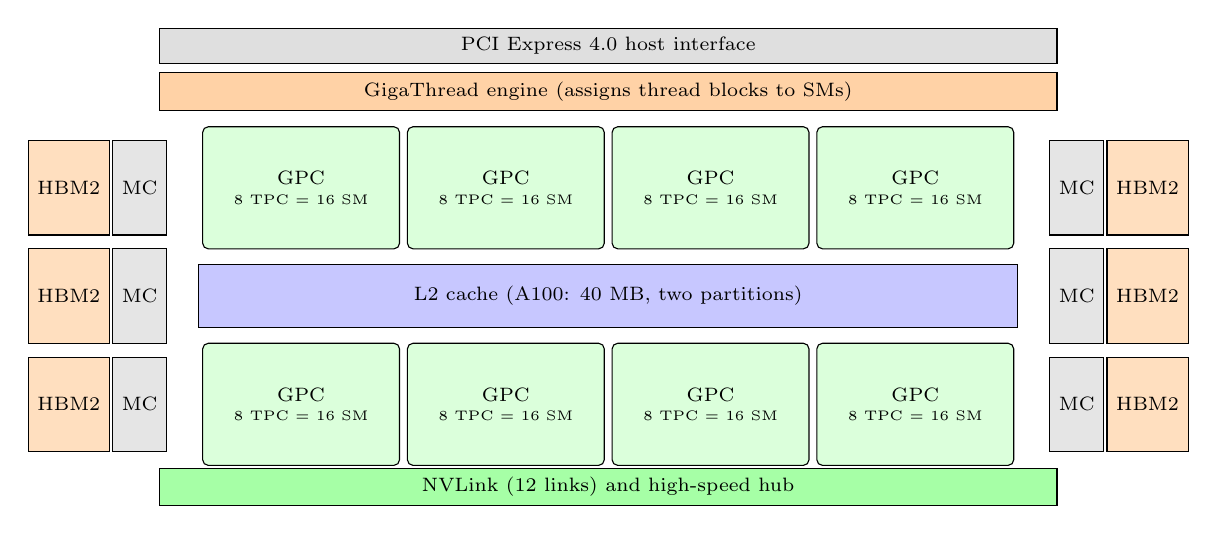
\begin{tikzpicture}[x=1cm,y=1cm,font=\scriptsize,
  gpc/.style={draw,rounded corners=2pt,fill=green!14,minimum width=2.5cm,minimum height=1.55cm,align=center},
  hbm/.style={draw,fill=orange!25,minimum width=1.0cm,minimum height=1.2cm,align=center},
  mc/.style={draw,fill=gray!20,minimum width=0.55cm,minimum height=1.2cm,align=center}]
  % top bars
  \node[draw,fill=gray!25,minimum width=11.4cm,minimum height=0.45cm] at (0,4.55) {PCI Express 4.0 host interface};
  \node[draw,fill=orange!35,minimum width=11.4cm,minimum height=0.45cm] at (0,3.97) {GigaThread engine (assigns thread blocks to SMs)};
  % GPCs top row and bottom row
  \foreach \i in {0,1,2,3}{
    \node[gpc] at (-3.9+2.6*\i,2.75) {GPC\\[-1pt]{\tiny 8 TPC $=$ 16 SM}};
    \node[gpc] at (-3.9+2.6*\i,0.0) {GPC\\[-1pt]{\tiny 8 TPC $=$ 16 SM}};
  }
  % L2
  \node[draw,fill=blue!22,minimum width=10.4cm,minimum height=0.8cm] at (0,1.375) {L2 cache (A100: 40 MB, two partitions)};
  % memory controllers and HBM left/right
  \foreach \y in {2.75,1.375,0}{
    \node[mc] at (-5.95,\y) {MC};
    \node[mc] at (5.95,\y) {MC};
    \node[hbm] at (-6.85,\y) {HBM2};
    \node[hbm] at (6.85,\y) {HBM2};
  }
  % NVLink
  \node[draw,fill=green!35,minimum width=11.4cm,minimum height=0.45cm] at (0,-1.05) {NVLink (12 links) and high-speed hub};
\end{tikzpicture}
\caption{Simplified block diagram of the full GA100 chip. The A100 product enables $7$ of the $8$ GPCs
(and not all TPCs inside them) and $5$ of the $6$ HBM2 stacks. Compare slide~5.}
\label{fig:gpu}
\end{figure}
